\documentclass[11pt]{beamer} 
\usetheme{cwc} 

\usepackage{amsmath,amssymb}
\usepackage{graphicx,acronym,setspace,epstopdf,pdflscape}
\usepackage{subeqnarray,multirow,cite,array,color,mathtools,setspace,geometry}

\acrodef{MSE}{mean squared error}
\acrodef{IBC}{interference broadcast channel}
\acrodef{MC}{multi-cell}
\acrodef{BS}{base station}
\acrodef{MIMO}{multiple-input multiple-output}
\acrodef{SISO}{single-input single-output}
\acrodef{MU}{multiple users}
\acrodef{OFDM}{orthogonal frequency division multiplexing}
\acrodef{WSRM}{weighted sum rate maximization}
\acrodef{QoS}{quality of service}
\acrodef{SCA}{successive convex approximation}
\acrodef{SNR}{signal-to-noise ratio}
\acrodef{MMSE}{minimum \acl{MSE}}
\acrodef{SIR}{signal-to-interference ratio}
\acrodef{SINR}{signal-to-interference-plus-noise ratio}
\acrodef{Q-WSRM}{queue \acl{WSRM}}
\acrodef{QM}{queue minimizing}
\acrodef{SRA}{spatial resource allocation}
\acrodef{JSFRA}{joint space-frequency resource allocation}
\acrodef{WMMSE}{weighted \acl{MMSE}}
\acrodef{KKT}{Karush-Kuhn-Tucker}
\acrodef{GP}{geometric programming}
\acrodef{SOC}{second-order cone}
%\acrodef{BCDM}{block coordinate descent method}
\acrodef{ADMM}{alternating directions method of multipliers}
\acrodef{PD}{primal decomposition}
\acrodef{DD}{dual decomposition}
\acrodef{FFR}{fractional frequency reuse}
\acrodef{DC}{difference of convex}
\acrodef{Q-WSRME}{\ac{Q-WSRM} extended}
\acrodef{TDD}{time division duplexing}
\acrodef{CSI}{channel state information}
\acrodef{AO}{alternating optimization}
\acrodef{OTA}{over-the-air}
\acrodef{PL}{path loss}
\acrodef{TDM}{time division multiplexing}
\acrodef{UC}{uncoordinated}
\acrodef{SoC}{system-on-chip}
\acrodef{WMMSE}{weighted minimum mean squared error}
\acrodef{AMBA}{Advanced Microcontroller Bus Architecture}
\acrodef{AXI}{Advanced Extensible Interface}
\acrodef{FPGA}{Field-programmable gate array}
\acrodef{MSMCSRAM}{multi-core shared memory}
\acrodef{IPC}{inter-processor communications}
\acrodef{CIC}{chip-level interrupt controller}
\acrodef{MCSDK}{multi-core software development kit}
\acrodef{AMP}{Asymmetric Multi-Processing}
\newcommand{\mbf}[1]{\mathbf{#1}}
\newcommand{\me}[1]{\( #1 \)}
\newcommand{\mc}[1]{\mathcal{#1}}
\newcommand{\fall}{\forall}
\newcommand{\set}[1]{\left \lbrace #1 \right \rbrace }
\newcommand{\mvec}[2]{\mathbf{#1}_{#2}}
\newcommand{\ith}[1]{{#1}^\mathrm{th}}
\newcommand{\pr}[1]{{#1}^\prime}
\newcommand{\mbfa}[1]{{\boldsymbol{#1}}}
\newcommand{\herm}{\mathrm{H}}
\newcommand{\sset}[1]{\left [ #1 \right ]}
\newcommand{\rfrac}[2]{{}^{#1}/{}_{#2}}
\newcommand{\eqspace}{\IEEEeqnarraynumspace}
\newcommand{\enoise}{\widetilde{N}_0}
\newcommand{\eqsub}{\IEEEyessubnumber}
\newcommand{\review}[1]{{\textcolor[rgb]{0 0 0.6}{#1}}}
\newcommand{\trace}{\mathrm{tr}}
\newcommand{\tran}{\mathrm{T}}
\newcommand{\R}[1]{\label{#1}\linelabel{#1}}
\newcommand{\lr}[1]{page~\pageref{#1}, line~\lineref{#1}}
\newcommand{\eqn}[1]{\(#1\)}
\newcommand{\mx}{\mbf{m}}
\newcommand{\my}{\mbf{w}}
\newcommand{\mz}{\mbfa{\gamma}}
\newcommand{\mxb}{{{\mbf{m}}}}
\newcommand{\myb}{{{\mbf{w}}}}
\newcommand{\iterate}[2]{{#1}^{(#2)}}
\newcommand{\iter}[3]{{#1}_{#2}^{(#3)}}
\newcommand{\ma}{\mbf{x}}

\graphicspath{{./../Figures/}}
\DeclareGraphicsExtensions{.pdf}

\epstopdfsetup{update,prepend,prefersuffix=false,suffix=}
\DeclareGraphicsRule{.eps}{pdf}{.pdf}{`epstopdf #1}
\pdfcompresslevel=9

\linespread{1.1}
\title{Exploiting Multi-Core SoC Architecture for \acs{MU-MIMO} Schedulers}
\author{{Ganesh Venkatraman, Janne Janhunen, and Markku Juntti} \\ \scriptsize{Email: \{gvenkatr, janne.janhunen, markku.juntti\}@ee.oulu.fi}}

\begin{document}

\begin{frame}
    \titlepage
\end{frame}

\begin{frame}{Outline} \scriptsize
    \tableofcontents
\end{frame}

\acused{BS} \acused{MIMO} \acused{OFDM}

\section{Abstract}

\begin{frame}{Abstract}
	\begin{itemize}
		\item \blutxt{Problem Studied - } Implementing multi-user MIMO scheduler schemes on \gretxt{TI TCI6636K2H eight core SoC}
		\item \blutxt{Issues addressed -}
			\begin{itemize}
				\item Complexity involved in implementing scheduling algorithms - \redtxt{low complex algorithm design}
				\item How to \redtxt{partition scheduler processing among eight cores} in \gretxt{TI TCI6636K2H eight core SoC}
			\end{itemize}
		\item \blutxt{Summary - } Proposed implementation \redtxt{supports up to \eqn{100} users in the system with \eqn{4 \times 4} MIMO configuration}
	\end{itemize}
\end{frame}

\section{Introduction}

\begin{frame}{Introduction and Motivation}
\begin{itemize}
\item Current standards are moving towards multi-antenna systems due to its numerous advantages
\item To avail the benefits, spatially multiplexing multiple user streams are considered
\item In order to do so, efficient precoding and user subset are to be identified
\item In this work, we analyze the computational needs of different MU-MIMO scheduling algorithms for a single scheduling block
\item We evaluate algorithm complexity by implementing on \gretxt{TI TCI6636K2H eight core SoC}
\end{itemize}
\end{frame}

\section{System Model \& Assumptions}

\begin{frame}{Notations used}
\begin{itemize}
\item We consider a single-cell multi-user \ac{MIMO} scenario
\item Let \me{K} be the total number of users with \me{N_R} antenna elements
\item Let \me{\kappa} be the total available spatial streams for a user \me{k}, given by \me{\kappa = \min (N_T,N_R)}
\item \eqn{\mvec{H}{\hat{k}} \in \mathbb{C}^{N_R \times N_T}} be the channel between \ac{BS} and user \eqn{\hat{k}, \forall k \in \mc{U}}
\item Let \eqn{\mc{A} \subset \mc{U}} be the subset of users chosen by scheduling algorithm
\end{itemize}
\end{frame}

\begin{frame}{System Model}
\begin{itemize}
\item Let \eqn{\mvec{H}{\hat{k}} = \mvec{U}{\hat{k}} \mvec{D}{\hat{k}} \mvec{V}{\hat{k}}^\herm} be singular value decomposition of \eqn{\mvec{H}{\hat{k}}}
\item Let \eqn{k = \kappa \hat{k} + i} be the virtual user corresponding to the spatial stream \eqn{i \in \{0,\dotsc,\kappa-1\}}
\item Using this, we denote virtual channel \eqn{\mvec{h}{k} = \mvec{U}{\hat{k}}(i)^\herm \mvec{H}{\hat{k}}}, where \eqn{\mvec{U}{\hat{k}}(i)} corresponds to the column \eqn{i} of \eqn{\mvec{U}{\hat{k}}}
\item Now, the received symbol \eqn{\hat{d}_k} of virtual user \eqn{k} is given as
\[\hat{d}_k = \mvec{h}{k} \mvec{m}{k} d_k + \sum_{i \in \mc{A} \backslash \{k\}} \mvec{h}{k} \mvec{m}{i} d_i + {n}_{k}\]
\item where \me{\mvec{m}{k} \in \mathbb{C}^{N_T \times 1}} is the transmit precoder of user \me{k}
\end{itemize}
\end{frame}

\section{Scheduling Algorithms}

\begin{frame}{Overview of Scheduling Algorithms}
\begin{itemize}
	\item To minimize interference, only a subset of users are allowed for transmission
	\item Subset selection with certain objective requires exhaustive search
	\item \redtxt{Scheduling can inherently be performed by precoder designs} - efficient iterative algorithms are available
	\item However, as the user count increases, complexity scales up significantly
	\item Hence, precoders are to be designed only for a subset of users chosen by scheduling algorithms
\end{itemize}
\end{frame}

\subsection{Successive Projections}

\begin{frame}{Successive Projections\eqn{^\dagger}}
\begin{itemize}
\item Based on \redtxt{Gram-Schmidt Orthogonalization} Procedure
\item In each iteration, user channel vectors are projected on to the subspace orthogonal to the span of channel vectors already chosen
\item Upon \blutxt{projecting on to the orthogonal subspace}, resulting vector with maximum norm is chosen as the candidate user
\[\mbf{N}(\mathcal{A}) = \mbf{I}_{N_T} - \mbf{F} \left (\mbf{F}^\herm \mbf{F} \right )^{-1} \mbf{F}^\herm\]
\item where \eqn{\mbf{F}} is the matrix formed by stacking channel vector of already chosen users in \eqn{\mc{A}}
\end{itemize}
\eqn{^\dagger}\scriptsize{T. Yoo and A. Goldsmith, "{On the Optimality of Multi-Antenna Broadcast Scheduling using zero-forcing Beamforming},” in \emph{IEEE J. Sel. Areas Commun.}, vol. 24, no. 3. IEEE, march 2006.}
\end{frame}

\subsection{Product of Independent Projections}

\begin{frame}{Product of Independent Projections (PIPD)\eqn{^\dagger}}
	\begin{itemize}
	\item As compared to the subspace projection in previous algorithm, \blutxt{vector projections} are considered
	\item Each user channel is projected on to unit vector in the direction of already chosen users channel
	\item Selection is based on the product of independent vector projections
	\item Performs significantly closer to successive projections method
	\item Due to vector projections, inverse calculation is not required - \redtxt{low complexity}
	\end{itemize}
\eqn{^\dagger}\scriptsize{Venkatraman, G., Tolli, A., Janhunen, J., and Juntti, M. "Low Complexity Multi-User MIMO Scheduling for Weighted Sum Rate Maximization", in \emph{Proc. of European Signal Process. Conference (EUSIPCO)}, pp. 820--824, 2013}
\end{frame}

\subsection{Block Diagram \& Performance Figure}

\begin{landscape}
\begin{frame}[plain]
	\begin{figure}
		\centering
		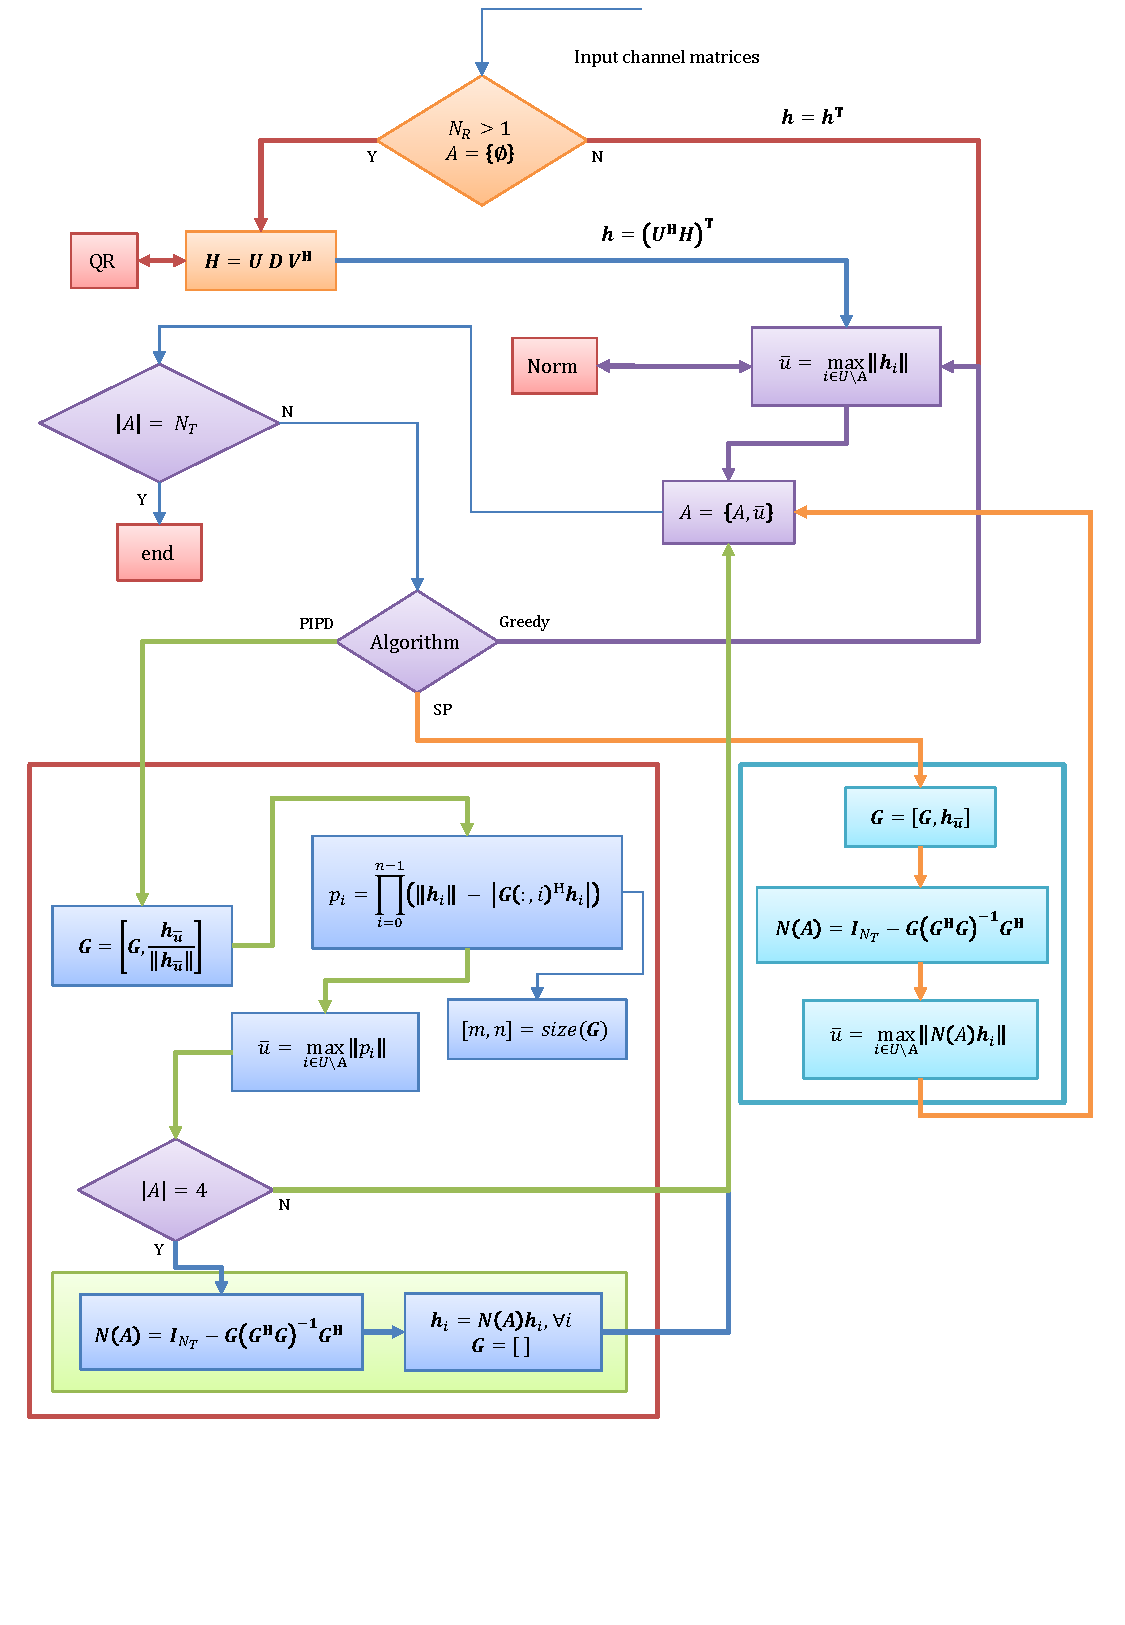
\includegraphics[trim=0.5in 1.5in 0in 1in,width=\columnwidth, angle=0]{Algorithm_Model}
		\caption{Block diagram of the scheduler algorithms: greedy, PIPD and successive projections}
	\end{figure}
\end{frame}
\end{landscape}

\begin{frame}
\begin{figure}
	\centering
	\caption{Comparison of Scheduler Algorithms for $K = 100$ users.}
	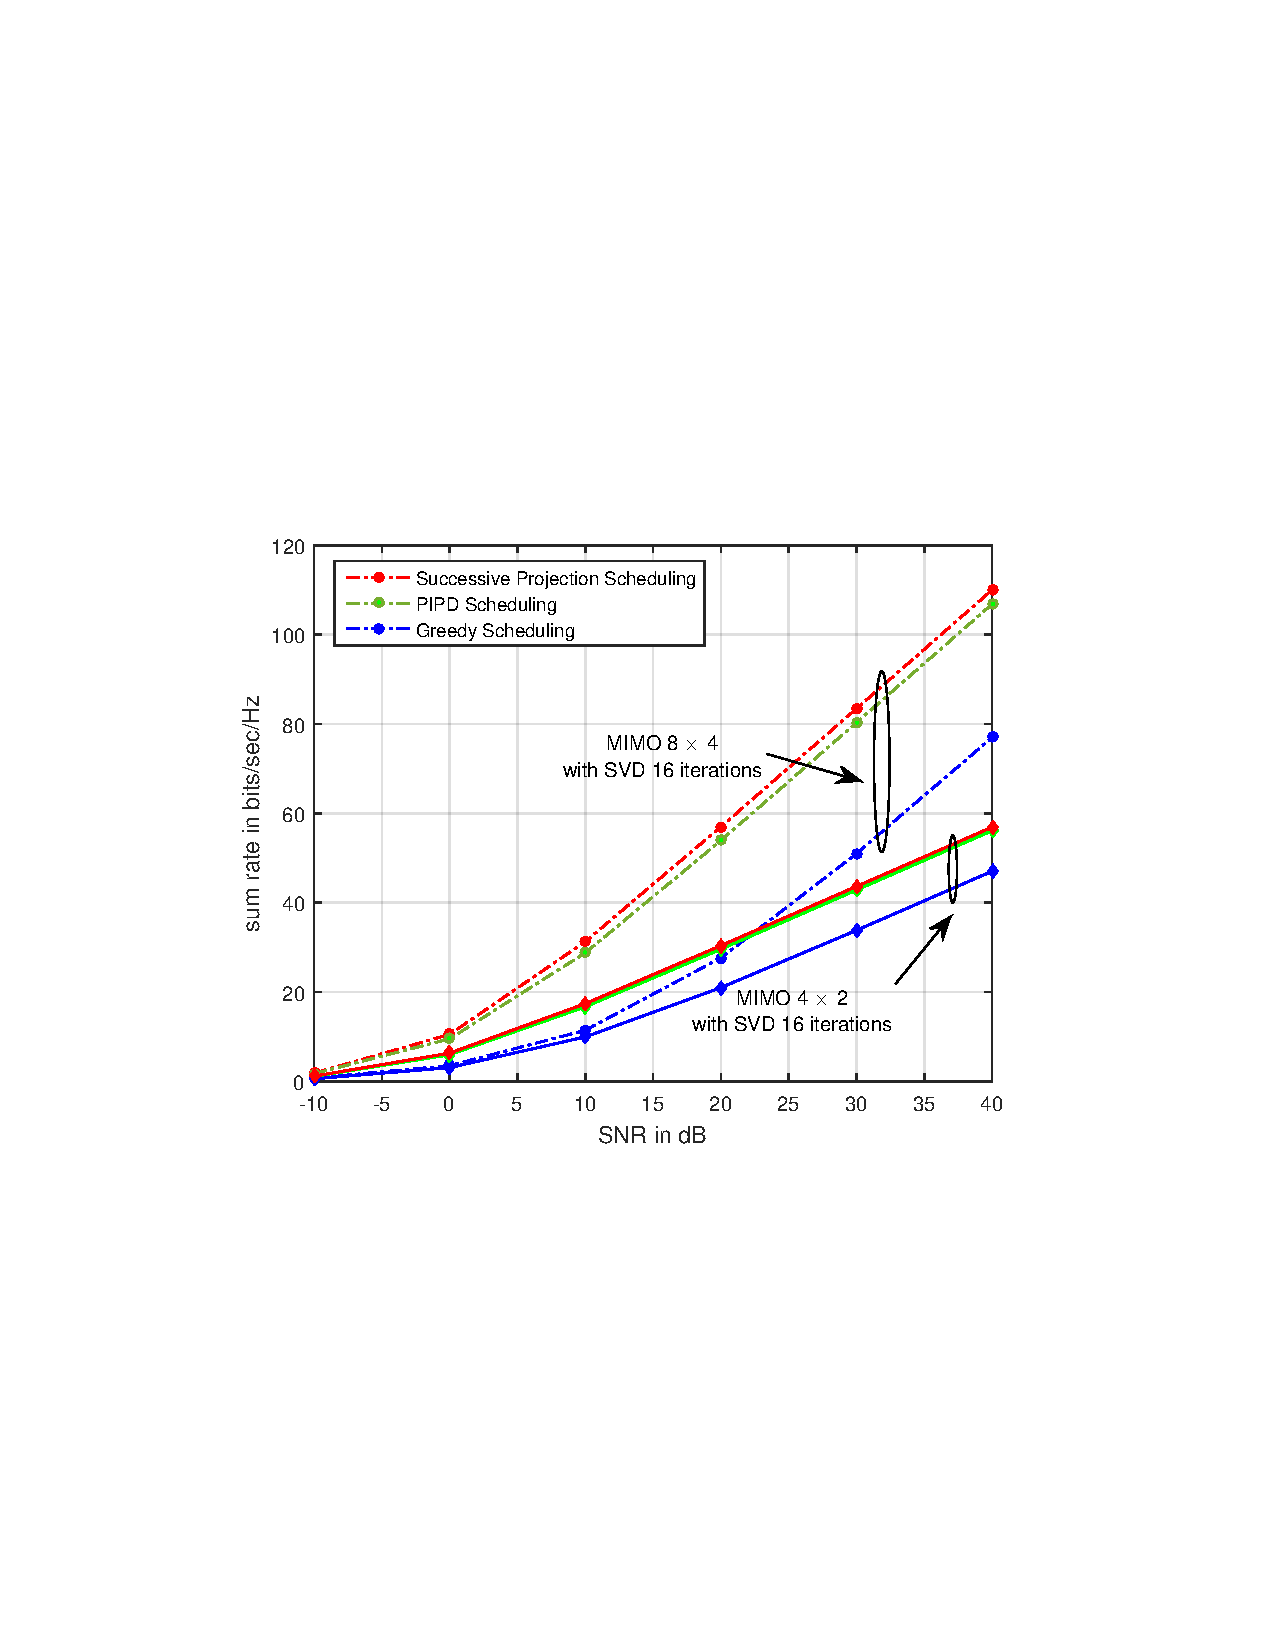
\includegraphics[trim=1.5in 3.5in 1.5in 3.5in,width=0.8\columnwidth]{sra_100}
\end{figure}
\end{frame}

\section{TIC6636K2H Implementation}

\subsection{Overview of TIC6636K2H Eight Core SoC}

\begin{frame}{Overview of TIC6636K2H Eight Core SoC}
	\begin{itemize}
		\item Four ARM Cortex A15 operating at \@ \eqn{1.4}GHz
		\item Eight C66x CorePacs DSP Core Subsystems \@ \eqn{1.2}GHz
		\item 1024K Byte Local L2 Per CorePac
		\item 6 MB MSM SRAM Memory Shared by DSP CorePacs and ARM CorePac
		\item TeraNet Fabric interconnect between core subsystems and peripherals
		\item DDR3 memory interface
	\end{itemize}
\end{frame}

\begin{frame}{Partitioning of Algorithm}
	\begin{itemize}
		\item Computationally, SVD is the most demanding operation
		\item SVD is performed by \blutxt{repeated QR factorization} (16 iterations)
		\item In order to utilize the SoC efficiently, \redtxt{SVD is shared among eight C66x cores}
		\item SVD processing begins with a \blutxt{chip level interrupt controller (CIC) interrupt} from Core(0)
		\item Channel matrices are \gretxt{stored in MSM SRAM memory}, which is accessible to all C66x cores
		\item Upon completion, Core(0) carries out scheduler design until completion
	\end{itemize}
\end{frame}

\begin{frame}{Implementation of Scheduler Algorithm}
	\begin{itemize}
		\item Each core runs \blutxt{separate copy of SYS-BIOS}
		\item Inter core communication is facilitated using MCSDK 3.0 software stack
		\item Storage address of the channel buffer in MSM SRAM is fixed across cores using \gretxt{\textrm{\#pragma location}}
		\item \redtxt{Avoids the usage of \textit{SharedMem} and \textit{Notify} modules} to attain the same
		\item \blutxt{\textit{IPC} module is used to synchronize} the cores upon {BIOS\_Start()} function call
	\end{itemize}
\end{frame}

\begin{frame}{Core(0) Implementation}
	\begin{itemize}
		\item \redtxt{Signed Q1.15 format} for real and imaginary entries
		\item \gretxt{CIC interrupt from Core (0)} is used to notify the \blutxt{availability of channel buffer to other cores}
		\item \redtxt{Cache \textit{write-back}} is performed upon completing SVD processing by all cores
		\item Upon completion, \gretxt{Core (0) proceeds with scheduling algorithm processing}
		\item However, in a dynamic scenario, \blutxt{CIC interrupt can be used to notify the completion from other cores}
		\item Number of SVD's per core - 
		\begin{itemize}
			\item Core(0) - \eqn{\left \lfloor \dfrac{K}{N_C} \right \rfloor + \left ( K - \left \lfloor \dfrac{K}{N_C} \right \rfloor \times N_C \right ) }
			\item Other cores - \eqn{\left \lfloor \dfrac{K}{N_C} \right \rfloor}
		\end{itemize}
	\end{itemize}
\end{frame}

\begin{frame}
	\begin{figure}
		\centering
		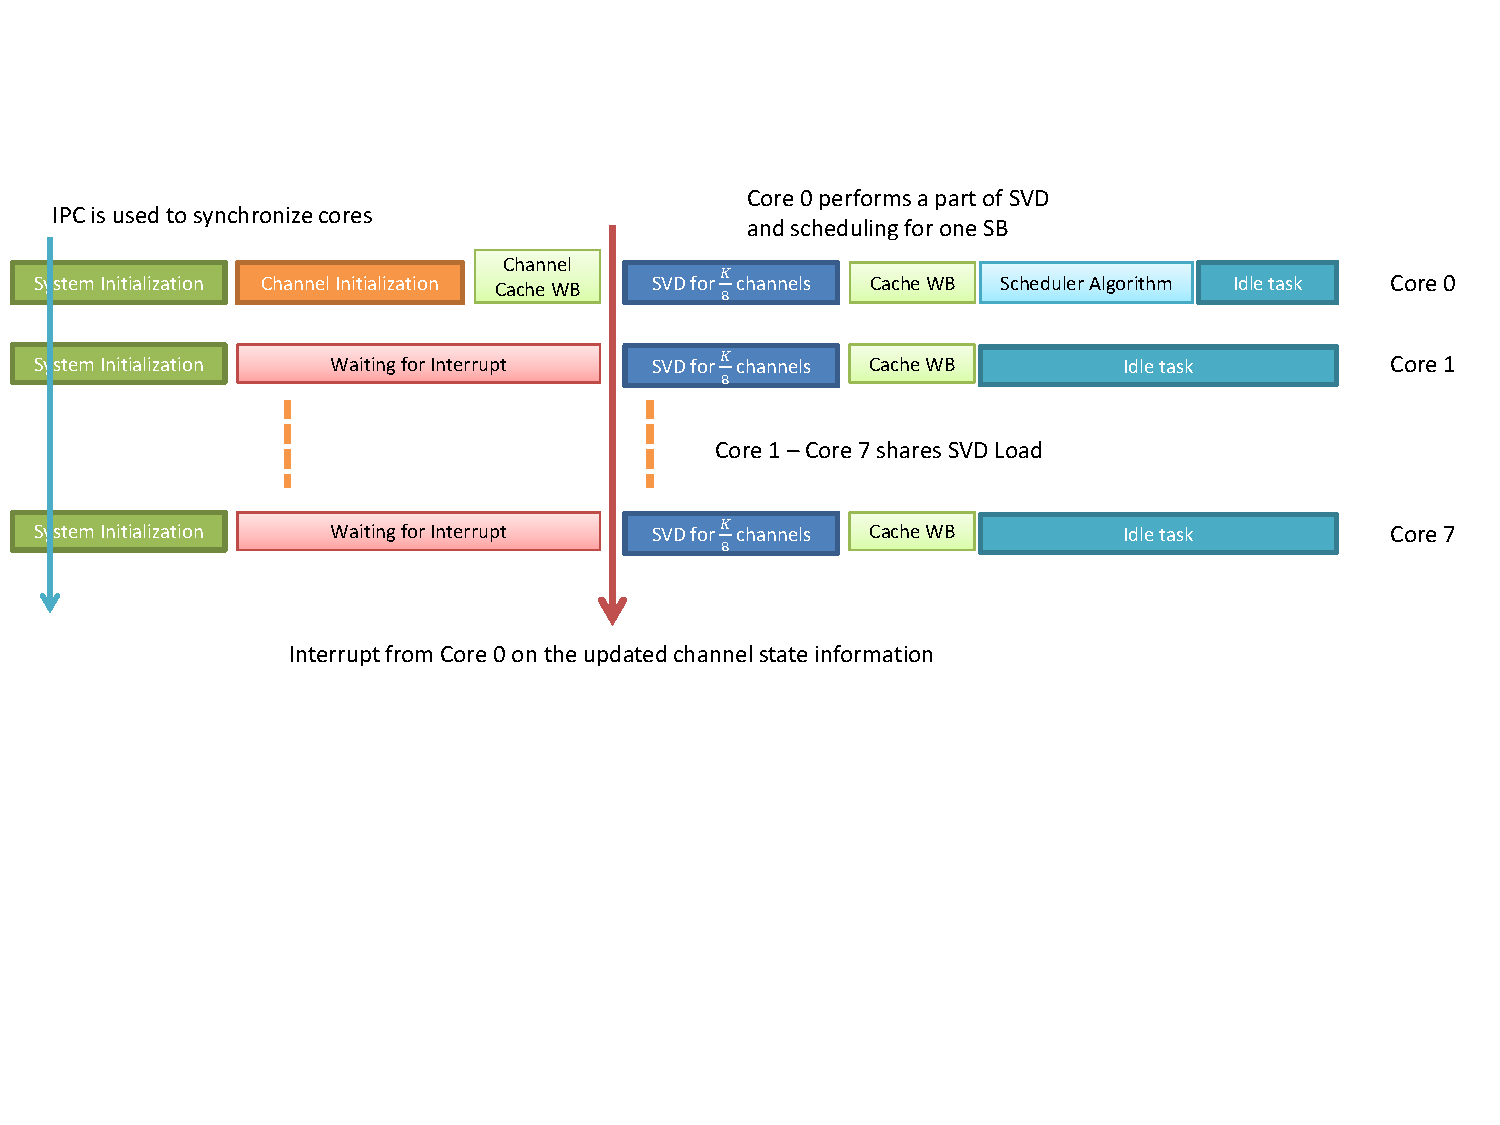
\includegraphics[trim=0in 2.25in 0in 1.0in,width=\columnwidth]{overall_scheduling}
		\caption{Task scheduling over \eqn{N_C = 8} cores.}
	\end{figure}
\end{frame}

\subsection{Complexity Analysis}

\begin{frame}
\begin{table} \caption{Scheduling Complexity for $K = 100$ users ($\mathrm{msec}$) with C66x operating at \eqn{1.2}GHz} \begin{center} \begin{tabular}{c c c c c c c}
			$N_T \times N_R $ & $\lambda$ & SVD \eqn{(1)} & SVD \eqn{(8)} & Greedy   & SP          & PIPD \\ 
			\hline \\
			$8 \times 4$ & 4 & 22.68 & 2.90 & 0.075 & 0.524 & 0.469 \\ 
			$8 \times 4$ & 2 & 22.68 & 2.90 & 0.064 & 0.325 & 0.268 \\
			$8 \times 2$ & 2 & 6.055 & 0.79 & 0.063 & 0.325 & 0.266 \\
			$8 \times 2$ & 1 & 6.055 & 0.79 & 0.058 & 0.226 & 0.166 \\
			\hline \\
			$4 \times 4$ & 4 & 15.81 & 2.07 & 0.045 & 0.168 & 0.167 \\ 
			$4 \times 4$ & 2 & 15.81 & 2.07 & 0.034 & 0.102 & 0.098 \\
			$4 \times 2$ & 2 & 4.844 & 0.64 & 0.034 & 0.102 & 0.097 \\
			$4 \times 2$ & 1 & 4.844 & 0.64 & 0.029 & 0.069 & 0.063 \\
			\hline \vspace{-0.3in}
		\end{tabular} \label{table:compexity_comparison}\end{center}
\end{table}
\end{frame}

\begin{frame}{Conclusion from Implementation Results}
	\begin{itemize}
		\item \gretxt{Current design can handle all scheduling algorithms} within \eqn{0.5} msec duration
		\item Moreover, with \blutxt{8 parallel cores}, it can \gretxt{support \eqn{8} scheduling blocks (SBs)} within \eqn{0.5} msec
		\item However, the complexity is mainly attributed by the SVD processing
		\item With current implementation, it can \blutxt{support the MIMO configuration of \eqn{8 \times 2} system for \eqn{K = 100} users}
		\item It is valid only \redtxt{if the channel changes onces in every radio frame} of \eqn{10} msec duration
		\item In \eqn{4 \times 2} configuration, current implementation supports \eqn{2} SBs using earlier assumption
	\end{itemize}
\end{frame}


\section{Conclusions}

\begin{frame}{Conclusions}
\begin{itemize}
\item We studied the implementation of different state-of-the-art MU-MIMO scheduling algorithms on TIC6636K2H
\item Complexity is mainly attributed to SVD decomposition of channel matrices
\item Using parallel implementation, current design can support \eqn{100} SVD of \eqn{8 \times 2} matrices in \eqn{6.055} msec
\item We have demonstrated that with the current implementation, \blutxt{all scheduling schemes meet the real-time requirements}
\item Even though we considered only single SB, the above implementation is scalable.
\end{itemize}
\end{frame}

\end{document}
